% ============================================================
%  Chapitre 2 : Logique et algebre de Boole
% ============================================================
\chapter{Logique et algèbre de Boole}
\chaptermark{Logique et algèbre de Boole}

\begin{quelqueslignes}
Chaque instruction d'un programme repose sur un test, chaque circuit d'un processeur sur un assemblage de portes, et l'un comme l'autre se décrivent avec les mêmes outils : les propositions, leurs tables de vérité et l'algèbre de Boole. Ce chapitre introduit les opérations logiques, étudie les énoncés conditionnels et biconditionnels, puis applique les connecteurs bit à bit aux mots machine. Il se termine par les portes logiques et les circuits, où le calcul booléen devient électronique. La logique des propositions demande aucune notion des chapitres précédents ; les opérations bit à bit en réutilisent l'écriture binaire.
\end{quelqueslignes}

\section{Opérations logiques}

\begin{definition}[proposition]
Une \emph{proposition} est un énoncé déclaratif qui est soit vrai, soit faux, mais jamais les deux à la fois. La valeur de vérité d'une proposition se note 1 lorsqu'elle est vraie et 0 lorsqu'elle est fausse ; une lettre comme $P$ ou $Q$ désigne une proposition indéterminée, appelée variable propositionnelle.
\end{definition}

Les phrases « Lomé est la capitale du Togo » (vraie), « 12 est divisible par 5 » (fausse) et « $x > 0$ » tant que $x$ n'est pas fixé : les deux premières sont des propositions, la troisième ne le devient qu'après avoir donné une valeur à $x$. Une question (« Quel est le plus grand diviseur de 16 ? »), une exclamation ou une ordre (« Fermez la session ! ») ne sont pas des propositions, car elles ne peuvent recevoir ni le vrai ni le faux.

\begin{definition}[table de vérité]
La \emph{table de vérité} d'une formule logique énumère toutes les attributions de valeurs possibles à ses lettres et donne, pour chacune, la valeur de la formule. Une formule à $n$ lettres a une table de $2^{n}$ lignes, chaque lettre valant 0 ou 1 indépendamment des autres.
\end{definition}

Les connecteurs construisent des propositions composées à partir de propositions simples. La \emph{négation} $\lnot P$ (« non $P$ ») est vraie lorsque $P$ est fausse. La \emph{conjonction} $P \land Q$ (« $P$ et $Q$ ») n'est vraie que si les deux le sont. La \emph{disjonction} $P \lor Q$ (« $P$ ou $Q$ ») est vraie dès que l'une l'est : le « ou » de l'informatique est inclusif. Le \emph{ou exclusif} $P \veebar Q$ (« $P$ ou bien $Q$ ») est vrai lorsque exactement l'une des deux l'est, comme le choix entre deux modes de paiement exclusifs. Le tableau~\ref{ch2:tab:connecteurs} fixe les valeurs des six connecteurs de base, dont l'implication $\rightarrow$ et l'équivalence $\leftrightarrow$ étudiées à la section suivante.

\begin{center}
\small
\begin{tabular}{C{0.75cm}C{0.75cm}C{0.95cm}C{1.15cm}C{1.05cm}C{1.15cm}C{1.35cm}C{1.55cm}}
\toprule
\rowcolor{robleuf}$P$ & $Q$ & $\lnot P$ & $P \land Q$ & $P \lor Q$ & $P \veebar Q$ & $P \rightarrow Q$ & $P \leftrightarrow Q$\\
\midrule
1 & 1 & 0 & 1 & 1 & 0 & 1 & 1\\
\rowcolor{rogrisf!50}1 & 0 & 0 & 0 & 1 & 1 & 0 & 0\\
0 & 1 & 1 & 0 & 1 & 1 & 1 & 0\\
\rowcolor{rogrisf!50}0 & 0 & 1 & 0 & 0 & 0 & 1 & 1\\
\bottomrule
\end{tabular}
\captionof{table}{Tables de vérité des six connecteurs usuels}
\label{ch2:tab:connecteurs}
\end{center}

\begin{exemple}[reconnaître et évaluer des propositions]
Parmi les énoncés suivants, seuls les trois premiers sont des propositions : « le bit 1 représente une tension haute » (vraie), « $2^{10} = 1000$ » (fausse, car $2^{10} = 1024$) et « si le fichier est corrompu, alors la sauvegarde restaure les données » (composée, dont la valeur dépend du fichier et de la sauvegarde). L'interrogative « le fichier est-il corrompu ? » et l'injonction « exécute le programme » n'en sont pas. Évaluons ensuite la formule $P \land \lnot Q$ avec $P$ : « le disque est plein » (vraie) et $Q$ : « la corbeille est vide » (fausse). On a $\lnot Q$ vraie, donc $P \land \lnot Q$ est vraie : le disque est plein et la corbeille n'est pas vide.
\end{exemple}

\begin{exemple}[table complète d'une formule à trois lettres]
Construisons la table de $(P \lor Q) \land R$. La formule a trois lettres : sa table compte $2^{3} = 8$ lignes, énumérées dans un ordre fixe, comme si l'on comptait de 0 à 7 en binaire. Les colonnes intermédiaires $P \lor Q$, puis $R$, puis la formule complète se calculent ligne par ligne.

\begin{center}
\begin{tabular}{C{0.7cm}C{0.7cm}C{0.7cm}C{1.4cm}C{1.2cm}C{2.2cm}}
\toprule
\rowcolor{robleuf}$P$ & $Q$ & $R$ & $P \lor Q$ & $R$ & $(P \lor Q) \land R$\\
\midrule
1 & 1 & 1 & 1 & 1 & 1\\
\rowcolor{rogrisf!50}1 & 1 & 0 & 1 & 0 & 0\\
1 & 0 & 1 & 1 & 1 & 1\\
\rowcolor{rogrisf!50}1 & 0 & 0 & 1 & 0 & 0\\
0 & 1 & 1 & 1 & 1 & 1\\
\rowcolor{rogrisf!50}0 & 1 & 0 & 1 & 0 & 0\\
0 & 0 & 1 & 0 & 1 & 0\\
\rowcolor{rogrisf!50}0 & 0 & 0 & 0 & 0 & 0\\
\bottomrule
\end{tabular}
\captionof{table}{Table à $2^{3} = 8$ lignes de la formule $(P \lor Q) \land R$}
\label{ch2:tab:troislettres}
\end{center}

La lecture est immédiate : la formule vaut 1 exactement sur les trois lignes où $R$ vaut 1 \emph{et} où l'un au moins de $P$, $Q$ vaut 1. Le nombre de lignes double à chaque lettre ajoutée : quatre lettres donnent 16 lignes, dix lettres donnent 1024 lignes : c'est pourquoi les méthodes algébriques de la section 6 deviennent indispensables.
\end{exemple}

\section{Énoncés conditionnels et biconditionnels}

\begin{definition}[implication]
L'\emph{implication} $P \rightarrow Q$, qui se lit « si $P$ alors $Q$ », est fausse uniquement dans le cas où $P$ est vraie et $Q$ fausse. $P$ en est l'\emph{hypothèse}, $Q$ la \emph{conclusion}. Lorsque l'hypothèse est fausse, l'implication est vraie : « si un octet vaut plus que 255, alors le réseau est saturé » ne peut être contredite par aucun octet réel.
\end{definition}

À toute implication on attache deux autres implications. La \emph{réciproque} de $P \rightarrow Q$ est $Q \rightarrow P$, qui échange hypothèse et conclusion ; la \emph{contraposée} est $\lnot Q \rightarrow \lnot P$, qui garde l'ordre mais nie les deux membres. Prenons $P$ : « la figure est un carré » et $Q$ : « la figure a quatre côtés ». L'implication $P \rightarrow Q$ est vraie ; sa réciproque est fausse, car un rectangle a quatre côtés sans être un carré ; sa contraposée « si la figure n'a pas quatre côtés, alors ce n'est pas un carré » est vraie. Le tableau~\ref{ch2:tab:recip} montre que la contraposée a exactement la même table que l'implication, alors que la réciproque s'en distingue :

\begin{center}
\begin{tabular}{C{0.8cm}C{0.8cm}C{1.8cm}C{1.8cm}C{2.4cm}}
\toprule
\rowcolor{robleuf}$P$ & $Q$ & $P \rightarrow Q$ & $Q \rightarrow P$ & $\lnot Q \rightarrow \lnot P$\\
\midrule
1 & 1 & 1 & 1 & 1\\
\rowcolor{rogrisf!50}1 & 0 & 0 & 1 & 0\\
0 & 1 & 1 & 0 & 1\\
\rowcolor{rogrisf!50}0 & 0 & 1 & 1 & 1\\
\bottomrule
\end{tabular}
\captionof{table}{Implication, réciproque et contraposée : les colonnes 3 et 5 coïncident}
\label{ch2:tab:recip}
\end{center}

\begin{definition}[biconditionnel]
L'\emph{équivalence} (ou biconditionnel) $P \leftrightarrow Q$, qui se lit « $P$ si et seulement si $Q$ », est vraie lorsque $P$ et $Q$ ont la même valeur de vérité. Elle exprime que les deux implications se tiennent à la fois : $P \leftrightarrow Q \equiv (P \rightarrow Q) \land (Q \rightarrow P)$.
\end{definition}

Dire « un fichier s'ouvre si et seulement s'il n'est pas corrompu », c'est affirmer ensemble les deux sens : un fichier non corrompu s'ouvre, et un fichier qui s'ouvre n'est pas corrompu. Il suffit qu'un seul des deux sens tombe pour que le biconditionnel tombe.

\begin{exemple}[le raisonnement de l'accusé]
Un raisonnement classique rapporte l'argument suivant : « l'accusé n'a pu se rendre coupable que s'il était à New York à 18 heures le 1\ier{} janvier ; or il a été établi qu'il était à ce moment-là à Washington ; il n'est donc pas coupable ». Posons $C$ : « l'accusé est coupable » et $N$ : « il était à New York à 18 heures le 1\ier{} janvier ». La première phrase se traduit par $C \rightarrow N$, l'observation par $\lnot N$ (être à Washington exclut d'être à New York à cet instant), et la conclusion par $\lnot C$. Le raisonnement entier s'écrit $\bigl((C \rightarrow N) \land \lnot N\bigr) \rightarrow \lnot C$, et sa table à $2^2 = 4$ lignes se calcule colonne par colonne :

\begin{center}
\begin{tabular}{C{0.8cm}C{0.8cm}C{1.7cm}C{1.1cm}C{2.9cm}C{1.0cm}C{3.2cm}}
\toprule
\rowcolor{robleuf}$C$ & $N$ & $C \rightarrow N$ & $\lnot N$ & $(C \rightarrow N) \land \lnot N$ & $\lnot C$ & formule complète\\
\midrule
1 & 1 & 1 & 0 & 0 & 0 & 1\\
\rowcolor{rogrisf!50}1 & 0 & 0 & 1 & 0 & 0 & 1\\
0 & 1 & 1 & 0 & 0 & 1 & 1\\
\rowcolor{rogrisf!50}0 & 0 & 1 & 1 & 1 & 1 & 1\\
\bottomrule
\end{tabular}
\captionof{table}{Le raisonnement de l'accusé : la dernière colonne ne contient que des 1}
\label{ch2:tab:accuse}
\end{center}

La dernière colonne ne contient que des 1 : le raisonnement est \emph{valide}, quelles que soient les vérités effectives de $C$ et de $N$. La logique ne dit pas si l'accusé est coupable ; elle garantit que, si les prémisses tiennent, la conclusion s'impose.
\end{exemple}

\begin{exemple}[de la phrase à la formule]
Traduisons deux énoncés d'un règlement de salle informatique. Première phrase : « si l'étudiant a payé sa contribution, alors il accède au réseau ». Posons $P$ : « l'étudiant a payé sa contribution » et $Q$ : « il accède au réseau » ; la phrase se traduit par $P \rightarrow Q$, dont la réciproque $Q \rightarrow P$ (« s'il accède au réseau, c'est qu'il a payé ») n'est pas automatiquement vraie, l'accès pouvant exister par d'autres voies. Seconde phrase : « l'étudiant imprime si et seulement si son compte est crédité » ; posons $I$ : « l'étudiant imprime » et $C$ : « son compte est crédité » ; elle se traduit par $I \leftrightarrow C$, c'est-à-dire $(I \rightarrow C) \land (C \rightarrow I)$ : sans crédit, pas d'impression, et toute impression prouve un crédit.
\end{exemple}

En programmation, l'implication se matérialise par l'instruction conditionnelle « SI \ldots{} ALORS \ldots{} FINSI » (dite « IF \ldots{} THEN » en anglais). Le fragment qui lit un nombre et le multiplie par 2 lorsqu'il est positif et impair s'écrit :
\begin{center}
\texttt{LIRE x} \quad \texttt{SI x > 0 ET x impair ALORS} \quad \texttt{y = 2 * x} \quad \texttt{FINSI}
\end{center}
La condition du SI est elle-même une proposition composée : « $x > 0$ » et « $x$ est impair » sont reliées par un ET logique, exactement au sens du tableau~\ref{ch2:tab:connecteurs}. La machine n'exécute le bloc ALORS que lorsque cette condition vaut 1 ; les tests d'un programme se conçoivent et se déboguent ainsi avec les mêmes tables de vérité que le reste du chapitre.

\section{Les opérations bit à bit}

Un processeur applique les connecteurs non plus à des propositions, mais directement aux bits de deux mots de même longueur : chaque position est traitée indépendamment des autres, c'est l'\emph{opération bit à bit}. Ces opérations servent à forcer, tester ou masquer certains bits d'un mot sans toucher aux autres, ce qui en fait l'outil quotidien de la programmation système.

\begin{exemple}[évaluation bit à bit de deux mots de huit bits]
Soient $P = 01100111$ et $Q = 11110001$ deux mots de huit bits. On aligne les deux mots et l'on calcule position par position.

\begin{center}
\begin{tabular}{L{2.6cm}C{0.65cm}C{0.65cm}C{0.65cm}C{0.65cm}C{0.65cm}C{0.65cm}C{0.65cm}C{0.65cm}}
\toprule
\rowcolor{robleuf}\textbf{Mot ou opération} & \multicolumn{8}{c}{bits, lus de gauche à droite}\\
\midrule
$P$ & 0 & 1 & 1 & 0 & 0 & 1 & 1 & 1\\
\rowcolor{rogrisf!50}$Q$ & 1 & 1 & 1 & 1 & 0 & 0 & 0 & 1\\
$P \land Q$ & 0 & 1 & 1 & 0 & 0 & 0 & 0 & 1\\
\rowcolor{rogrisf!50}$P \lor Q$ & 1 & 1 & 1 & 1 & 0 & 1 & 1 & 1\\
$P \veebar Q$ & 1 & 0 & 0 & 1 & 0 & 1 & 1 & 0\\
\bottomrule
\end{tabular}
\captionof{table}{Opérations bit à bit sur $P = 01100111$ et $Q = 11110001$}
\label{ch2:tab:bits}
\end{center}

Détaillons deux positions. En position 1, $P$ vaut 0 et $Q$ vaut 1 : le produit logique vaut $0 \land 1 = 0$, la somme logique $0 \lor 1 = 1$ et l'ou exclusif $0 \veebar 1 = 1$. En position 6, $P$ vaut 1 et $Q$ vaut 0 : on obtient $1 \land 0 = 0$, $1 \lor 0 = 1$ et $1 \veebar 0 = 1$. Le tableau donne ainsi $P \land Q = 01100001$, $P \lor Q = 11110111$ et $P \veebar Q = 10010110$.

Ces opérations deviennent de vrais outils lorsqu'on les applique avec un \emph{masque}, un mot binaire choisi pour n'agir que sur certaines positions. Effectuer $M \land 0000\,1111$ conserve les quatre bits de droite de $M$ et met les autres à zéro : c'est la lecture d'un demi-octet. Effectuer $M \lor 0000\,0001$ force le bit de droite à 1 sans toucher aux autres ; effectuer $M \veebar 0000\,0001$ le bascule, le changeant en son contraire. Tester, forcer, basculer : les trois gestes élémentaires de la programmation système reposent sur ce triplet.
\end{exemple}

\begin{exemple}[chiffrement d'un message par le ou exclusif]
Le ou exclusif est sa propre réciproque : pour tout bit $a$, $a \veebar a = 0$ et $a \veebar 0 = a$, si bien que combiner deux fois un mot avec la même clé le restitue : $(M \veebar K) \veebar K = M$. Si $M$ est un message en binaire et $K$ une clé de même longueur, le message chiffré est $C = M \veebar K$, et le destinataire retrouve $M$ en appliquant la même opération avec la même clé. Chiffrons $M = 1011\,0100\,1111\,0001$ avec la clé $K = 1010\,1110\,0100\,1110$ :
\begin{center}
\begin{tabular}{rcl}
$M$ & $=$ & \texttt{1011 0100 1111 0001}\\
$K$ & $=$ & \texttt{1010 1110 0100 1110}\\
$C = M \veebar K$ & $=$ & \texttt{0001 1010 1011 1111}\\
\end{tabular}
\qquad
\begin{tabular}{rcl}
$C$ & $=$ & \texttt{0001 1010 1011 1111}\\
$K$ & $=$ & \texttt{1010 1110 0100 1110}\\
$C \veebar K$ & $=$ & \texttt{1011 0100 1111 0001} $= M$\\
\end{tabular}
\end{center}
Détaillons le premier groupe : $1 \veebar 1 = 0$, $0 \veebar 0 = 0$, $1 \veebar 1 = 0$, $1 \veebar 0 = 1$, d'où $0001$ ; les autres groupes se traitent de même. Le déchiffrement par la même clé restitue le message initial : c'est le principe du chiffrement à clé symétrique, où une même clé secrète sert à chiffrer puis à déchiffrer.
\end{exemple}

\begin{remarque}[le bit de parité]
Le ou exclusif fournit aussi un contrôle d'erreur élémentaire. On ajoute à un mot binaire un \emph{bit de parité} choisi pour que le nombre total de 1 soit pair ; le récepteur recompte : si le total devient impair, au moins un bit a changé en route, et le message est rejeté. Le contrôle repose sur la propriété $a \veebar a = 0$ : le ou exclusif de tous les bits du mot correct vaut 0, et toute erreur bascule le résultat à 1. Ce contrôle simple, dit VRC, détecte toute erreur impaire et équipe encore les liaisons série les plus modestes.
\end{remarque}

\section{Circuits et portes logiques}

\begin{definition}[porte logique]
Une \emph{porte logique} est un composant électronique élémentaire qui réalise une fonction logique : elle reçoit des états d'entrée codés par des niveaux de tension (0 ou 1) et produit une sortie imposée, pour chaque combinaison d'entrées, par la table de vérité de la fonction réalisée.
\end{definition}

\begin{center}
\small
\begin{tabular}{L{2.1cm}L{1.9cm}L{3.6cm}L{7.0cm}}
\toprule
\rowcolor{robleuf}\textbf{Porte} & \textbf{Nom anglais} & \textbf{Expression} & \textbf{Sorties pour $AB = 00, 01, 10, 11$}\\
\midrule
ET & AND & $S = A \cdot B$ & $0\ 0\ 0\ 1$\\
\rowcolor{rogrisf!50}OU & OR & $S = A + B$ & $0\ 1\ 1\ 1$\\
NON & NOT & $S = \overline{A}$ (une entrée) & $1$ pour $A = 0$ ; $0$ pour $A = 1$\\
\rowcolor{rogrisf!50}NON-ET & NAND & $S = \overline{A \cdot B}$ & $1\ 1\ 1\ 0$\\
NON-OU & NOR & $S = \overline{A + B}$ & $1\ 0\ 0\ 0$\\
\rowcolor{rogrisf!50}OU exclusif & XOR & $S = A \veebar B$ & $0\ 1\ 1\ 0$\\
\bottomrule
\end{tabular}
\captionof{table}{Les six portes logiques de base, leur expression et leurs sorties}
\label{ch2:tab:portes}
\end{center}

Chaque porte possède un symbole graphique normalisé, reconnaissable à sa silhouette : la porte ET a un côté gauche plat pour les entrées et un côté droit arrondi ; la porte OU a la forme d'un bouclier à pointe arrondie ; la porte NON est un triangle suivi d'un petit cercle d'inversion ; les portes NAND et NOR reprennent les silhouettes du ET et du OU avec le même cercle en sortie. La figure~\ref{ch2:fig:circuit} montre le circuit analysé dans l'exemple suivant : un inverseur, deux portes ET et une porte OU.

\begin{center}
\begin{tikzpicture}[line width=0.9pt]
  % --- entree B et inverseur ---
  \node[anchor=east] at (-0.7,3.2) {$B$};
  \draw (-0.65,3.2) -- (0.3,3.2);
  \draw (0.3,2.95) -- (0.3,3.45) -- (0.75,3.45) -- (0.75,2.95) -- cycle;
  \draw (0.9,3.2) circle (0.15);
  \draw (1.05,3.2) -- (2.75,3.2);
  \node[font=\scriptsize, text=rogris, anchor=south] at (1.9,3.26) {$\overline{B}$};
  % --- entree C ---
  \node[anchor=east] at (-0.7,2.6) {$C$};
  \draw (-0.65,2.6) -- (2.75,2.6);
  % --- porte ET du haut : NON B . C ---
  \draw (2.75,2.6) -- (2.75,3.2) -- (3.35,3.2)
        arc[start angle=90, end angle=-90, radius=0.3] -- (2.75,2.6);
  \draw (3.65,2.9) -- (4.45,2.9);
  \node[font=\scriptsize, text=rogris, anchor=south] at (4.22,2.98) {$\overline{B} \cdot C$};
  % --- entrees A et B ---
  \node[anchor=east] at (-0.7,1.3) {$A$};
  \draw (-0.65,1.3) -- (2.75,1.3);
  \node[anchor=east] at (-0.7,0.7) {$B$};
  \draw (-0.65,0.7) -- (2.75,0.7);
  % --- porte ET du bas : A . B ---
  \draw (2.75,0.7) -- (2.75,1.3) -- (3.35,1.3)
        arc[start angle=90, end angle=-90, radius=0.3] -- (2.75,0.7);
  \draw (3.65,1.0) -- (4.45,1.0);
  \node[font=\scriptsize, text=rogris, anchor=south] at (4.25,1.08) {$A \cdot B$};
  % --- porte OU finale ---
  \draw (4.45,2.9) .. controls (4.73,2.55) and (4.73,1.35) .. (4.45,1.0);
  \draw (4.45,2.9) .. controls (5.15,2.75) and (5.45,2.15) .. (5.5,1.95);
  \draw (4.45,1.0) .. controls (5.15,1.15) and (5.45,1.75) .. (5.5,1.95);
  \draw (5.5,1.95) -- (6.1,1.95);
  \node[anchor=west] at (6.15,1.95) {$F$};
\end{tikzpicture}
\captionof{figure}{Circuit réalisant $F = A \cdot B + \overline{B} \cdot C$ : un inverseur, deux ET et un OU}
\label{ch2:fig:circuit}
\end{center}

\begin{center}
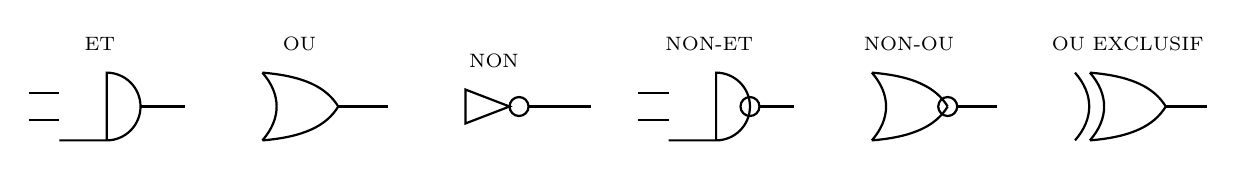
\begin{tikzpicture}[line width=0.8pt, scale=0.86, every node/.style={font=\scriptsize}]
  % ET
  \begin{scope}
    \draw (0,0) -- (0.7,0) -- (0.7,1.0) arc[start angle=90, end angle=-90, radius=0.5] -- (0,0);
    \draw (-0.45,0.7) -- (0,0.7); \draw (-0.45,0.3) -- (0,0.3);
    \draw (1.2,0.5) -- (1.85,0.5);
    \node[anchor=south] at (0.6,1.18) {ET};
  \end{scope}
  % OU
  \begin{scope}[xshift=3.0cm]
    \draw (0,0) .. controls (0.28,0.32) and (0.28,0.68) .. (0,1.0);
    \draw (0,1.0) .. controls (0.62,0.95) and (0.95,0.78) .. (1.12,0.5);
    \draw (0,0) .. controls (0.62,0.05) and (0.95,0.22) .. (1.12,0.5);
    \draw (1.12,0.5) -- (1.85,0.5);
    \node[anchor=south] at (0.55,1.18) {OU};
  \end{scope}
  % NON
  \begin{scope}[xshift=6.0cm]
    \draw (0,0.25) -- (0,0.75) -- (0.65,0.5) -- cycle;
    \draw (0.79,0.5) circle (0.14);
    \draw (0.93,0.5) -- (1.85,0.5);
    \node[anchor=south] at (0.42,0.92) {NON};
  \end{scope}
  % NON-ET
  \begin{scope}[xshift=9.0cm]
    \draw (0,0) -- (0.7,0) -- (0.7,1.0) arc[start angle=90, end angle=-90, radius=0.5] -- (0,0);
    \draw (-0.45,0.7) -- (0,0.7); \draw (-0.45,0.3) -- (0,0.3);
    \draw (1.2,0.5) circle (0.14); \draw (1.34,0.5) -- (1.85,0.5);
    \node[anchor=south] at (0.6,1.18) {NON-ET};
  \end{scope}
  % NON-OU
  \begin{scope}[xshift=12.0cm]
    \draw (0,0) .. controls (0.28,0.32) and (0.28,0.68) .. (0,1.0);
    \draw (0,1.0) .. controls (0.62,0.95) and (0.95,0.78) .. (1.12,0.5);
    \draw (0,0) .. controls (0.62,0.05) and (0.95,0.22) .. (1.12,0.5);
    \draw (1.12,0.5) circle (0.14); \draw (1.26,0.5) -- (1.85,0.5);
    \node[anchor=south] at (0.55,1.18) {NON-OU};
  \end{scope}
  % OU EXCLUSIF
  \begin{scope}[xshift=15.0cm]
    \draw (0,0) .. controls (0.28,0.32) and (0.28,0.68) .. (0,1.0);
    \draw (0.22,0) .. controls (0.50,0.32) and (0.50,0.68) .. (0.22,1.0);
    \draw (0.22,1.0) .. controls (0.84,0.95) and (1.17,0.78) .. (1.34,0.5);
    \draw (0.22,0) .. controls (0.84,0.05) and (1.17,0.22) .. (1.34,0.5);
    \draw (1.34,0.5) -- (1.95,0.5);
    \node[anchor=south] at (0.78,1.18) {OU EXCLUSIF};
  \end{scope}
\end{tikzpicture}
\captionof{figure}{Les six silhouettes de portes : le cercle en sortie marque l'inversion}
\label{ch2:fig:portes}
\end{center}

\begin{exemple}[analyse du circuit $F = A \cdot B + \overline{B} \cdot C$]
Décrivons le circuit de la figure~\ref{ch2:fig:circuit} porte par porte : le fil $B$ traverse l'inverseur qui produit $\overline{B}$ ; la porte ET du bas reçoit $A$ et $B$ et produit $A \cdot B$ ; la porte ET du haut reçoit $\overline{B}$ et $C$ et produit $\overline{B} \cdot C$ ; la porte OU finale réunit les deux produits et fournit $F = A \cdot B + \overline{B} \cdot C$. La table du circuit se construit en une colonne par fil :

\begin{center}
\begin{tabular}{C{0.9cm}C{0.9cm}C{0.9cm}C{1.3cm}C{1.4cm}C{1.6cm}C{1.1cm}}
\toprule
\rowcolor{robleuf}$A$ & $B$ & $C$ & $\overline{B}$ & $A \cdot B$ & $\overline{B} \cdot C$ & $F$\\
\midrule
0 & 0 & 0 & 1 & 0 & 0 & 0\\
\rowcolor{rogrisf!50}0 & 0 & 1 & 1 & 0 & 1 & 1\\
0 & 1 & 0 & 0 & 0 & 0 & 0\\
\rowcolor{rogrisf!50}0 & 1 & 1 & 0 & 0 & 0 & 0\\
1 & 0 & 0 & 1 & 0 & 0 & 0\\
\rowcolor{rogrisf!50}1 & 0 & 1 & 1 & 0 & 1 & 1\\
1 & 1 & 0 & 0 & 1 & 0 & 1\\
\rowcolor{rogrisf!50}1 & 1 & 1 & 0 & 1 & 0 & 1\\
\bottomrule
\end{tabular}
\captionof{table}{Table de vérité complète du circuit $F = A \cdot B + \overline{B} \cdot C$}
\label{ch2:tab:circuit}
\end{center}

Lisons la ligne $ABC = 101$ : $\overline{B} = 1$, $A \cdot B = 1 \cdot 0 = 0$ et $\overline{B} \cdot C = 1 \cdot 1 = 1$, d'où $F = 0 + 1 = 1$. Le tableau montre que $F$ vaut 1 exactement pour les lignes $001$, $101$, $110$ et $111$, celles où $A$ et $B$ valent 1 ensemble ou où $B$ vaut 0 pendant que $C$ vaut 1 : le circuit agit comme un aiguillage qui suit $A \cdot B$ lorsque $B$ vaut 1 et $\overline{B} \cdot C$ lorsque $B$ vaut 0.
\end{exemple}

\begin{exemple}[concevoir la fonction majoritaire]
Un système de vote à trois délégués valide une motion si au moins deux d'entre eux votent pour. Notons $A$, $B$, $C$ les trois votes (1 pour, 0 contre) et cherchons la fonction $M$ qui vaut 1 dès que deux entrées au moins valent 1. Les lignes favorables de la table sont $011$, $101$, $110$ et $111$ ; on écrit donc chaque ligne favorable comme un produit et l'on somme les produits :
\[
M = \overline{A} \cdot B \cdot C + A \cdot \overline{B} \cdot C + A \cdot B \cdot \overline{C} + A \cdot B \cdot C .
\]
Chaque produit vaut 1 sur exactement sa ligne, et leur somme couvre les quatre lignes favorables : c'est la \emph{forme canonique} de la fonction, où chaque terme correspond à une ligne de la table. Le circuit se dessine alors mécaniquement : un inverseur par lettre niée, quatre portes ET à trois entrées, une porte OU à quatre entrées. On peut réduire cette première version par l'algèbre de la section 6 : en regroupant les termes deux à deux, $M$ se simplifie en $A \cdot B + A \cdot C + B \cdot C$, trois produits de deux entrées seulement, soit un circuit plus petit pour la même fonction.
\end{exemple}

\section{Propriétés des opérations logiques}

\begin{definition}[équivalence logique]
Deux formules $A$ et $B$ sont \emph{logiquement équivalentes}, noté $A \equiv B$, lorsqu'elles ont la même table de vérité : pour toute attribution de valeurs aux lettres, elles prennent la même valeur. Une \emph{tautologie} est une formule vraie sur toutes les lignes de sa table, une \emph{contradiction} une formule fausse sur toutes les lignes.
\end{definition}

\begin{propriete}[équivalences fondamentales]
Pour toutes propositions $P$, $Q$ et $R$ :
\begin{itemize}
  \item lois de De Morgan : $\lnot(P \lor Q) \equiv \lnot P \land \lnot Q$ \quad et \quad $\lnot(P \land Q) \equiv \lnot P \lor \lnot Q$ ;
  \item distributivités : $P \land (Q \lor R) \equiv (P \land Q) \lor (P \land R)$ \quad et \quad $P \lor (Q \land R) \equiv (P \lor Q) \land (P \lor R)$ ;
  \item implication : $P \rightarrow Q \equiv \lnot P \lor Q$ ; contraposée : $P \rightarrow Q \equiv \lnot Q \rightarrow \lnot P$ ;
  \item négation d'une implication : $\lnot(P \rightarrow Q) \equiv P \land \lnot Q$ ;
  \item double négation : $\lnot\lnot P \equiv P$ ; biconditionnel : $P \leftrightarrow Q \equiv (P \rightarrow Q) \land (Q \rightarrow P)$.
\end{itemize}
Chaque équivalence se vérifie en dressant les deux tables et en constatant qu'elles coïncident.
\end{propriete}

\begin{exemple}[l'implication se ramène au ou et à la négation]
Montrons $P \rightarrow Q \equiv \lnot P \lor Q$ par la table. On calcule les colonnes de $P \rightarrow Q$, de $\lnot P$ puis de $\lnot P \lor Q$ :

\begin{center}
\begin{tabular}{C{0.8cm}C{0.8cm}C{1.8cm}C{1.2cm}C{1.8cm}}
\toprule
\rowcolor{robleuf}$P$ & $Q$ & $P \rightarrow Q$ & $\lnot P$ & $\lnot P \lor Q$\\
\midrule
1 & 1 & 1 & 0 & 1\\
\rowcolor{rogrisf!50}1 & 0 & 0 & 0 & 0\\
0 & 1 & 1 & 1 & 1\\
\rowcolor{rogrisf!50}0 & 0 & 1 & 1 & 1\\
\bottomrule
\end{tabular}
\captionof{table}{Équivalence $P \rightarrow Q \equiv \lnot P \lor Q$ : les colonnes 3 et 5 coïncident}
\label{ch2:tab:impou}
\end{center}

Les colonnes 3 et 5 sont identiques ligne à ligne : l'équivalence est établie. Ce résultat permet d'exprimer l'implication avec les seuls connecteurs $\lor$ et $\lnot$, dont on verra qu'ils suffisent à construire tous les circuits.
\end{exemple}

\begin{exemple}[une contradiction et une tautologie]
Considérons $F_1 = P \land \lnot(P \lor Q)$, puis $F_2 = (P \land Q) \lor \lnot(P \land Q)$.

\begin{center}
\begin{tabular}{C{0.8cm}C{0.8cm}C{1.5cm}C{2.0cm}C{2.9cm}}
\toprule
\rowcolor{robleuf}$P$ & $Q$ & $P \lor Q$ & $\lnot(P \lor Q)$ & $P \land \lnot(P \lor Q)$\\
\midrule
1 & 1 & 1 & 0 & 0\\
\rowcolor{rogrisf!50}1 & 0 & 1 & 0 & 0\\
0 & 1 & 1 & 0 & 0\\
\rowcolor{rogrisf!50}0 & 0 & 0 & 1 & 0\\
\bottomrule
\end{tabular}
\captionof{table}{$P \land \lnot(P \lor Q)$ vaut 0 sur les quatre lignes : contradiction}
\label{ch2:tab:contra}
\end{center}

La formule $F_1$ affirme $P$ et, en même temps, la négation de $P \lor Q$, qui contient $P$ : elle se contredit elle-même et vaut 0 partout, c'est une \emph{contradiction}. La formule $F_2$, de structure $A \lor \lnot A$, affirme une chose ou sa négation sans troisième possibilité : sa table ne contient que des 1, c'est une \emph{tautologie} : c'est le principe du tiers exclu appliqué à la proposition $P \land Q$. Toute formule de la forme $A \lor \lnot A$ est ainsi une tautologie, et toute formule de la forme $A \land \lnot A$ une contradiction.
\end{exemple}

\begin{attention}
La négation d'une implication n'est pas l'implication des négations : $\lnot(P \rightarrow Q) \not\equiv \lnot P \rightarrow \lnot Q$. En français courant, « il est faux que, si j'ai le baccalauréat, je suis inscrit » ne signifie pas « si je n'ai pas le baccalauréat, je ne suis pas inscrit » : l'inscription peut avoir d'autres voies. La vraie négation est $P \land \lnot Q$ (j'ai le baccalauréat \emph{et} je ne suis pas inscrit), tandis que $\lnot P \rightarrow \lnot Q$ n'est autre que la réciproque de l'implication initiale.
\end{attention}

\begin{remarque}[De Morgan dans les programmes]
Les lois de De Morgan s'utilisent chaque fois qu'un programmeur écrit la négation d'une condition complexe. La négation de « le fichier existe \emph{et} il est lisible » n'est pas « le fichier n'existe pas et il n'est pas lisible », mais « le fichier n'existe pas \emph{ou} il n'est pas lisible » : $\lnot(P \land Q) \equiv \lnot P \lor \lnot Q$. En code, réécrire la condition sous la bonne forme évite des bugs subtils : un « ou » oublié dans une négation inverse complètement la logique du programme.
\end{remarque}

\section{Simplification booléenne}

Pour transformer les formules sans redresser des tables toujours plus grandes, George Boole (1815--1864) a proposé de manipuler le raisonnement au moyen d'équations : le vrai et le faux y deviennent les valeurs 1 et 0, le « et » une multiplication et le « ou » une addition. Claude Shannon a montré en 1938 que cette algèbre décrit exactement le comportement des circuits numériques : elle sert depuis en permanence, pour \emph{analyser} un circuit existant en écrivant son équation, et pour \emph{concevoir} la réalisation la plus simple d'une fonction voulue.

\begin{definition}[algèbre de Boole]
L'algèbre de Boole sur $\bits = \{0, 1\}$ comporte deux opérations binaires, la \emph{somme logique} $+$ (le « ou ») et le \emph{produit logique} $\cdot$ (le « et »), et une opération unaire, la \emph{complémentation} notée par une barre. Les postulats fixent le calcul sur 0 et 1.
\end{definition}

\begin{center}
\begin{tabular}{C{4.8cm}C{4.8cm}}
\toprule
\rowcolor{robleuf}\textbf{Produit logique ($\cdot$)} & \textbf{Somme logique ($+$)}\\
\midrule
$0 \cdot 0 = 0$ & $0 + 0 = 0$\\
\rowcolor{rogrisf!50}$0 \cdot 1 = 1 \cdot 0 = 0$ & $1 + 0 = 0 + 1 = 1$\\
$1 \cdot 1 = 1$ & $1 + 1 = 1$\\
\rowcolor{rogrisf!50}$\overline{0} = 1$ & $\overline{1} = 0$\\
\bottomrule
\end{tabular}
\captionof{table}{Les postulats de l'algèbre de Boole sur les éléments 0 et 1}
\label{ch2:tab:postulats}
\end{center}

Le seul postulat en désaccord avec l'arithmétique ordinaire est $1 + 1 = 1$ : la somme logique n'est pas l'addition binaire du chapitre 3, qui écrit $1 + 1 = 10$ avec un report. Les règles d'écriture suivent l'usage algébrique : le produit a préséance sur la somme ($a + b \cdot c$ se lit $a + (b \cdot c)$), le point de multiplication s'omet ($ab$ pour $a \cdot b$), et seules les parenthèses forcent un autre ordre. Le tableau~\ref{ch2:tab:theoremes} rassemble les théorèmes usuels, que l'on démontre par les axiomes ou par une table complète.

\begin{center}
\small
\begin{tabular}{L{3.2cm}L{6.0cm}L{6.0cm}}
\toprule
\rowcolor{robleuf}\textbf{Théorème} & \textbf{Forme somme} & \textbf{Forme produit}\\
\midrule
Élément absorbant & $a + 1 = 1$ & $a \cdot 0 = 0$\\
\rowcolor{rogrisf!50}Complémentation & $a + \overline{a} = 1$ & $a \cdot \overline{a} = 0$\\
Idempotence & $a + a = a$ & $a \cdot a = a$\\
\rowcolor{rogrisf!50}Absorption & $a + a \cdot b = a$ & $a \cdot (a + b) = a$\\
Simplification & $a + \overline{a} \cdot b = a + b$ & $a \cdot (\overline{a} + b) = a \cdot b$\\
\rowcolor{rogrisf!50}Involution & \multicolumn{2}{L{12.0cm}}{$\overline{\overline{a}} = a$}\\
Lois de De Morgan & $\overline{a + b} = \overline{a} \cdot \overline{b}$ & $\overline{a \cdot b} = \overline{a} + \overline{b}$\\
\bottomrule
\end{tabular}
\captionof{table}{Théorèmes usuels de l'algèbre de Boole ($a$, $b$ éléments de $\bits$)}
\label{ch2:tab:theoremes}
\end{center}

À titre de modèle, déroulons la démonstration algébrique de la seconde forme de l'absorption, chaque passage étant justifié par un axiome ou un théorème déjà acquis :
\[
\begin{array}{rcll}
a \cdot (a + b) &=& (a + 0) \cdot (a + b) & \text{élément neutre : } a = a + 0\\
&=& a + 0 \cdot b & \text{distributivité (seconde forme)}\\
&=& a + 0 & \text{élément absorbant : } b \cdot 0 = 0\\
&=& a . & \text{élément neutre. CQFD}
\end{array}
\]
Le dual $a + a \cdot b = a$ est acquis sans calcul, par le principe de dualité.

\begin{remarque}[le principe de dualité]
Chaque théorème du tableau~\ref{ch2:tab:theoremes} possède un \emph{dual} qui s'obtient en échangeant $+$ et $\cdot$, puis 0 et 1, sans toucher à la barre de complément : de l'idempotence $a + a = a$ on déduit $a \cdot a = a$, de l'absorbant $a + 1 = 1$ on déduit $a \cdot 0 = 0$. Dès qu'un résultat est prouvé, son dual est acquis, et les deux colonnes du tableau se mémorisent d'un même mouvement.
\end{remarque}

\begin{methode}[simplifier une expression booléenne]
\begin{enumerate}
  \item appliquer d'abord De Morgan pour faire descendre les barres sur les variables seules ;
  \item distribuer pour faire apparaître les paires $a \cdot \overline{a} = 0$ et $a + \overline{a} = 1$ ;
  \item réduire à l'aide de l'idempotence, de l'absorption et de la simplification $a + \overline{a} \cdot b = a + b$ ;
  \item contrôler en comparant les tables de l'expression initiale et du résultat sur quelques lignes, ou en re-dessinant le circuit réduit.
\end{enumerate}
\end{methode}

\begin{exemple}[simplifications algébriques pas à pas]
Simplifions $E_1 = (A + B) \cdot (A + \overline{B})$, puis $E_2 = \overline{A} \cdot B + A \cdot B + \overline{A} \cdot \overline{B}$.
\[
\begin{array}{rcll}
E_1 &=& A + B \cdot \overline{B} & \text{distributivité : } (a+b)(a+c) = a + bc\\
    &=& A + 0 & \text{complémentation}\\
    &=& A . & \text{élément neutre}
\end{array}
\]
Un circuit qui réalisait trois portes pour $E_1$ se réduit à un simple fil portant le signal $A$. Pour $E_2$, on groupe les deux premiers produits :
\[
\begin{array}{rcll}
E_2 &=& (\overline{A} + A) \cdot B + \overline{A} \cdot \overline{B} & \text{distributivité}\\
    &=& 1 \cdot B + \overline{A} \cdot \overline{B} & \text{complémentation}\\
    &=& B + \overline{A} \cdot \overline{B} & \text{élément neutre}\\
    &=& (B + \overline{A}) \cdot (B + \overline{B}) & \text{distributivité (seconde forme)}\\
    &=& (B + \overline{A}) \cdot 1 & \text{complémentation}\\
    &=& B + \overline{A} . & \text{élément neutre}
\end{array}
\]
L'expression initiale demandait trois ET, deux OU et deux inverseurs ; le résultat $B + \overline{A}$ s'obtient avec deux inverseurs et un OU. La fonction est inchangée, le circuit est plus petit, plus rapide et moins coûteux : c'est tout l'intérêt de la simplification booléenne.
\end{exemple}

\begin{exemple}[faire descendre une barre avec De Morgan]
Simplifions $F = \overline{\overline{A} + B} + A \cdot B$. La grande barre se traite d'abord par De Morgan :
\[
\overline{\overline{A} + B} = \overline{\overline{A}} \cdot \overline{B} = A \cdot \overline{B},
\]
en appliquant l'involution au complément double. Il reste $F = A \cdot \overline{B} + A \cdot B$, et la distributivité donne $F = A \cdot (\overline{B} + B) = A \cdot 1 = A$. Le contrôle par la table est immédiat : $F$ vaut 1 exactement lorsque $A$ vaut 1, quelle que soit la valeur de $B$, ce que l'expression initiale réalisait par un détour plus coûteux.
\end{exemple}

\begin{aretirer}
Une proposition est vraie ou fausse ; une formule à $n$ lettres a une table de $2^{n}$ lignes, et les six connecteurs usuels $\lnot$, $\land$, $\lor$, $\veebar$, $\rightarrow$, $\leftrightarrow$ ont leurs tables fixes (tableau~\ref{ch2:tab:connecteurs}). L'implication n'est fausse qu'en cas $1 \rightarrow 0$, sa contraposée $\lnot Q \rightarrow \lnot P$ a sa table, sa réciproque non ; le biconditionnel exprime la double implication. Les opérations bit à bit appliquent $\land$, $\lor$, $\veebar$ position par position, et le ou exclusif, propre inverse de lui-même, fonde le chiffrement à clé symétrique. En algèbre de Boole, $1 + 1 = 1$, et les théorèmes du tableau~\ref{ch2:tab:theoremes} (absorption, simplification, De Morgan) réduisent expressions et circuits. Toute cette panoplie se travaille à la séance de travaux dirigés 2, de la table complète au circuit réduit.
\end{aretirer}
